\documentclass[journal,10pt,onecolumn,compsoc]{IEEEtran}
\usepackage[margin=1.0in]{geometry} 
\usepackage{pdfpages} 
\usepackage{rotating}
\usepackage{tikz}
\graphicspath{/graphics} 
\setlength{\parskip}{\baselineskip} \setlength\parindent{24pt}
\usepackage[english]{babel}
%\usepackage{fullpage}
\title{WYSIWYG TensorFlow\texttrademark Project}
\author{Group 33: Behnam Saeedi, Connor Sedwick, Collin Dorsett \\ CS463 Senior Capstone}
\date{\today}

\begin{document}
\setcounter{page}{0}
\maketitle
\newpage
\setcounter{page}{0}
\tableofcontents
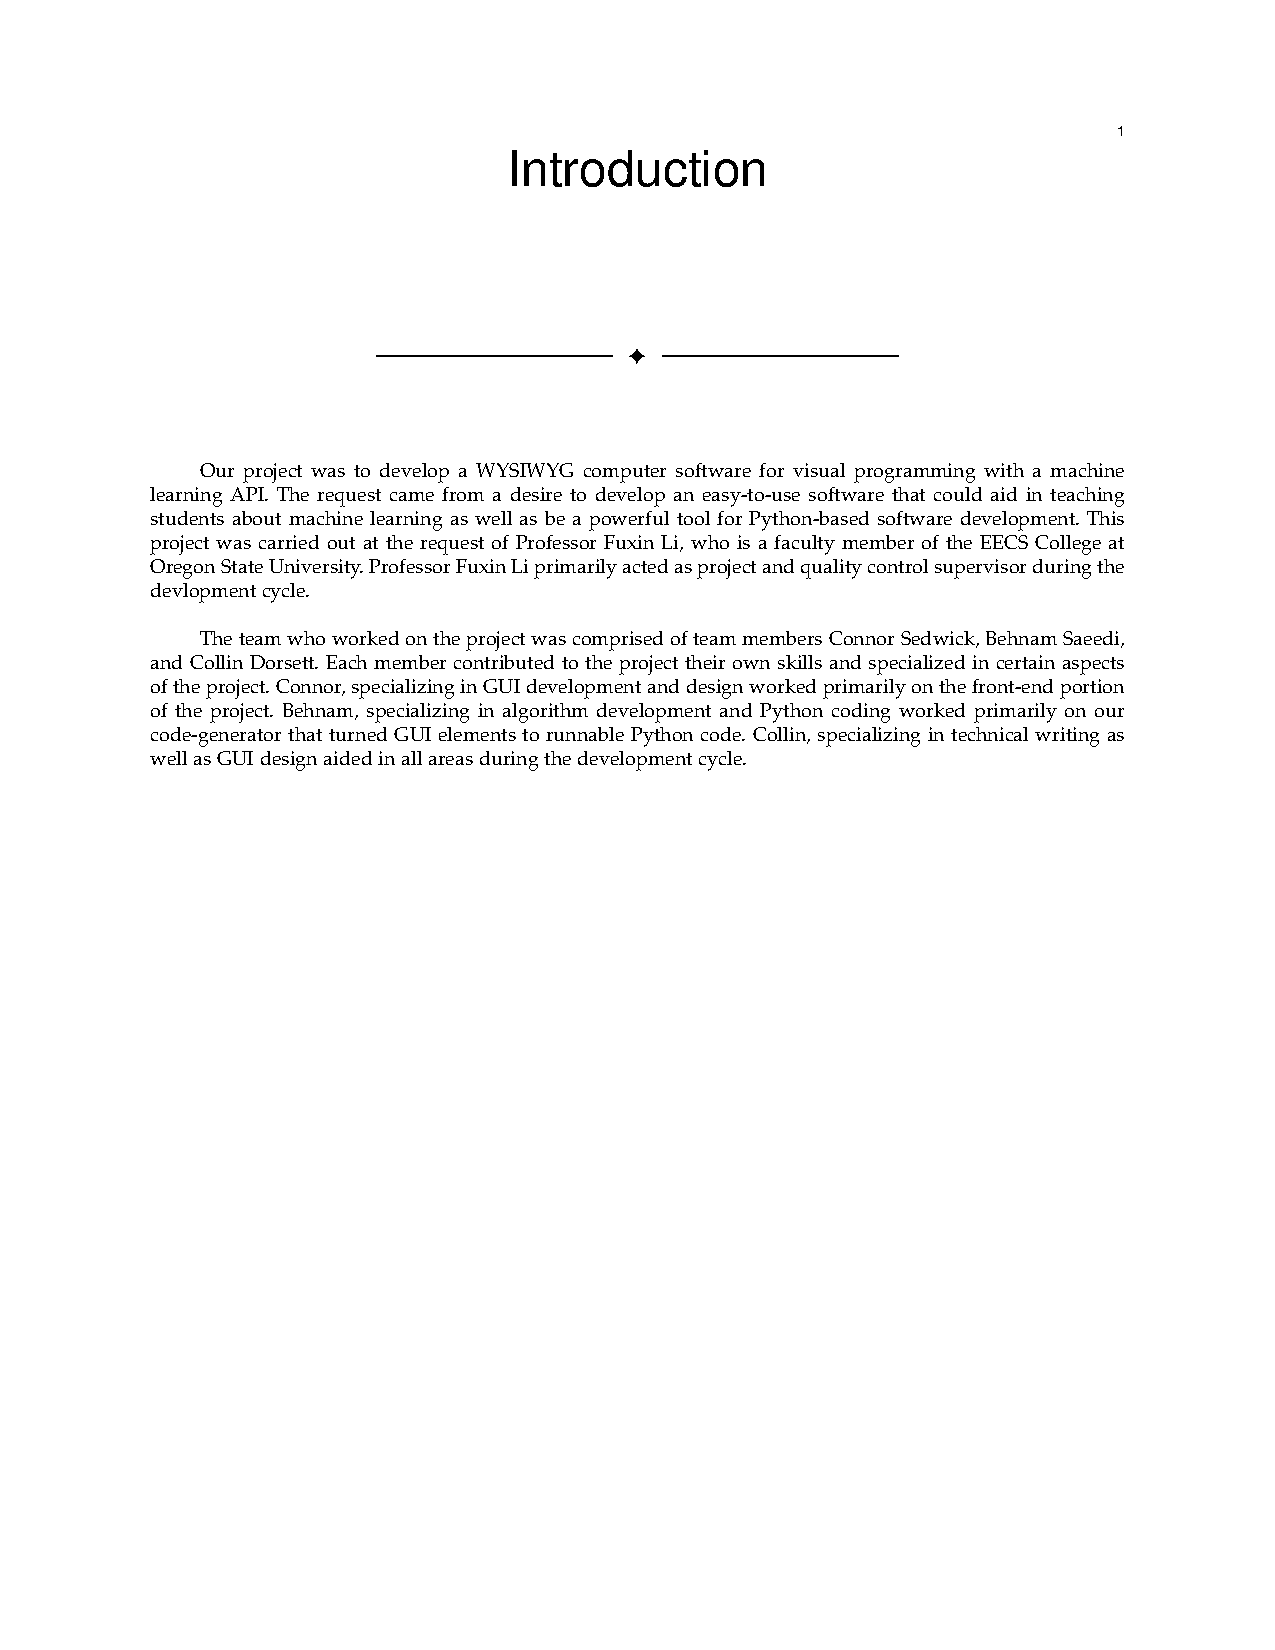
\includepdf[pages=1, addtotoc={1,section,1,Introduction,Introduction}]{introduction}

\includepdf[pages=1-, addtotoc={1,section,1,Requirements,Requirements}]{requirements-document-visualflow}
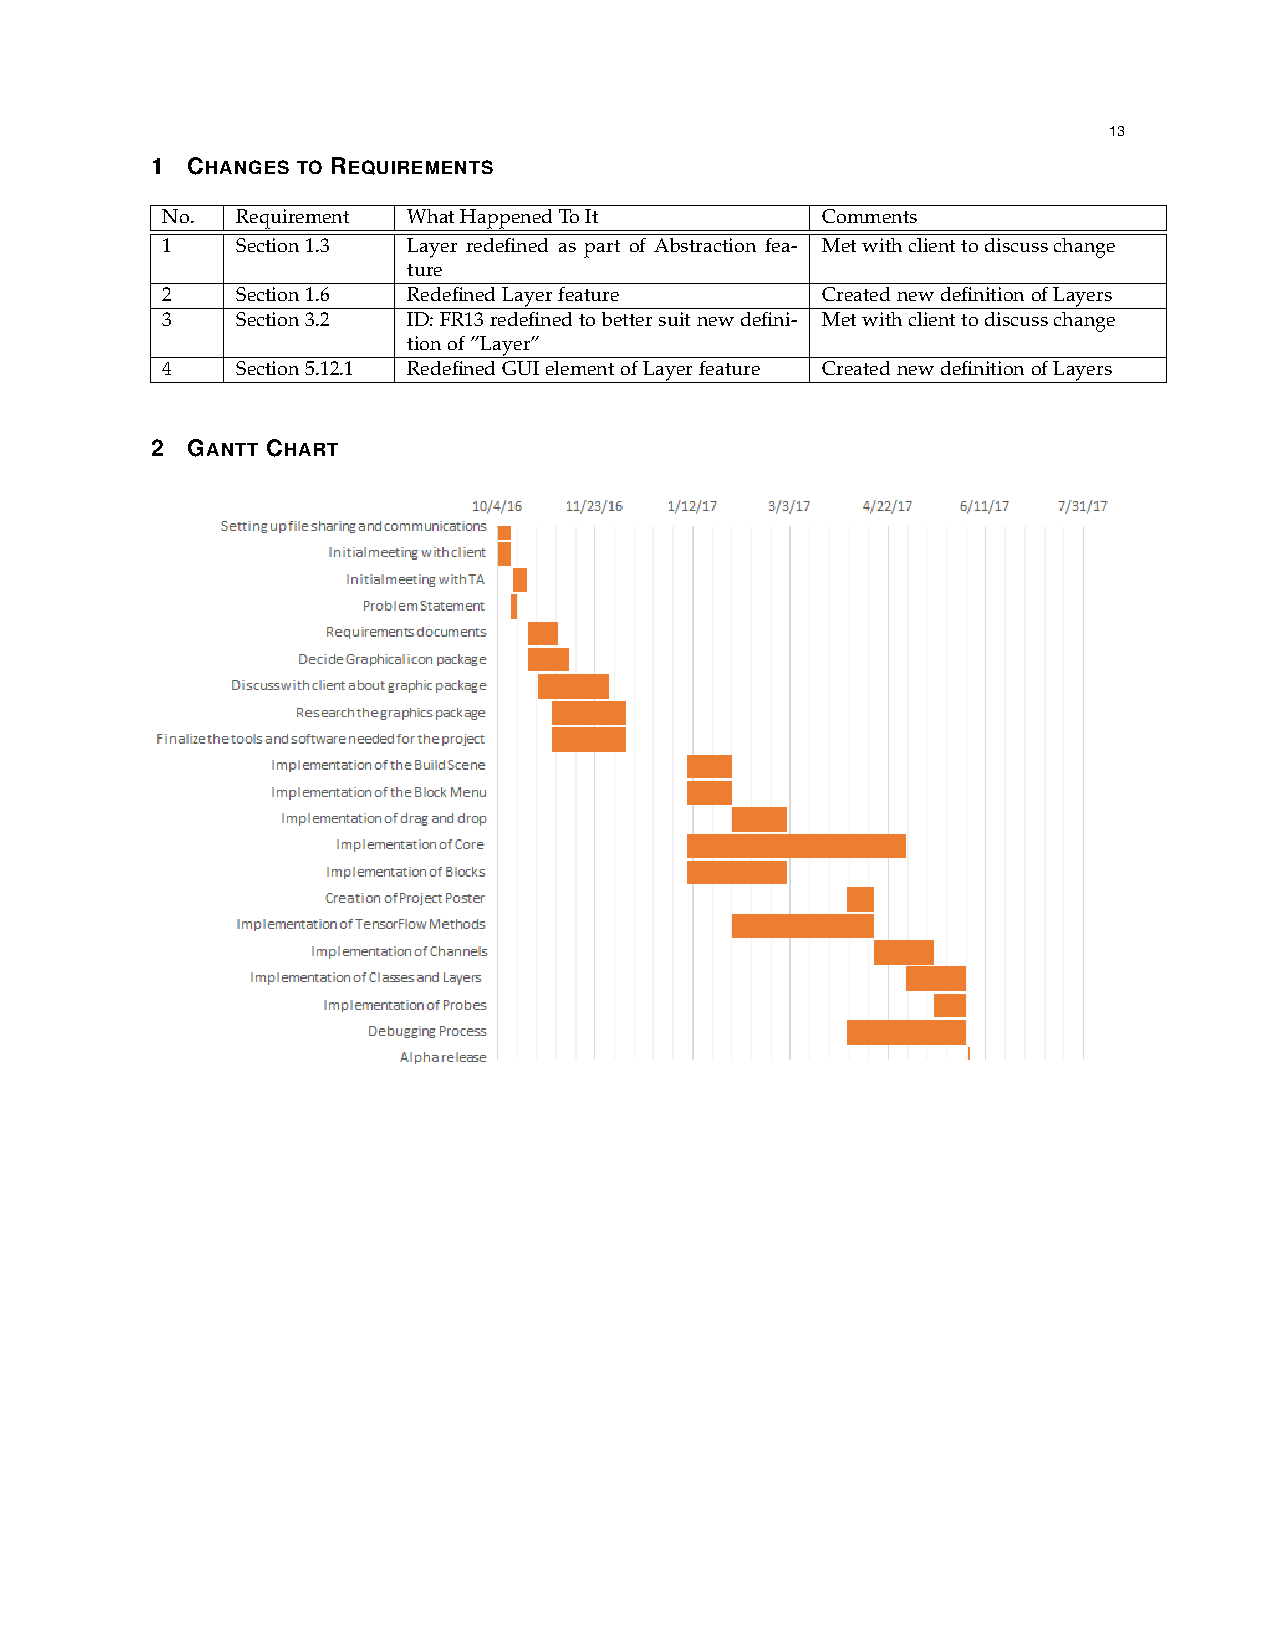
\includepdf[pages=1-, addtotoc={1,subsection,2,Changes to Requirements,Changes to Requirements}]{change-requirements-gantt}

\includepdf[pages=1-, addtotoc={1,section,1,Design Document,Design Document}]{Design_doc}
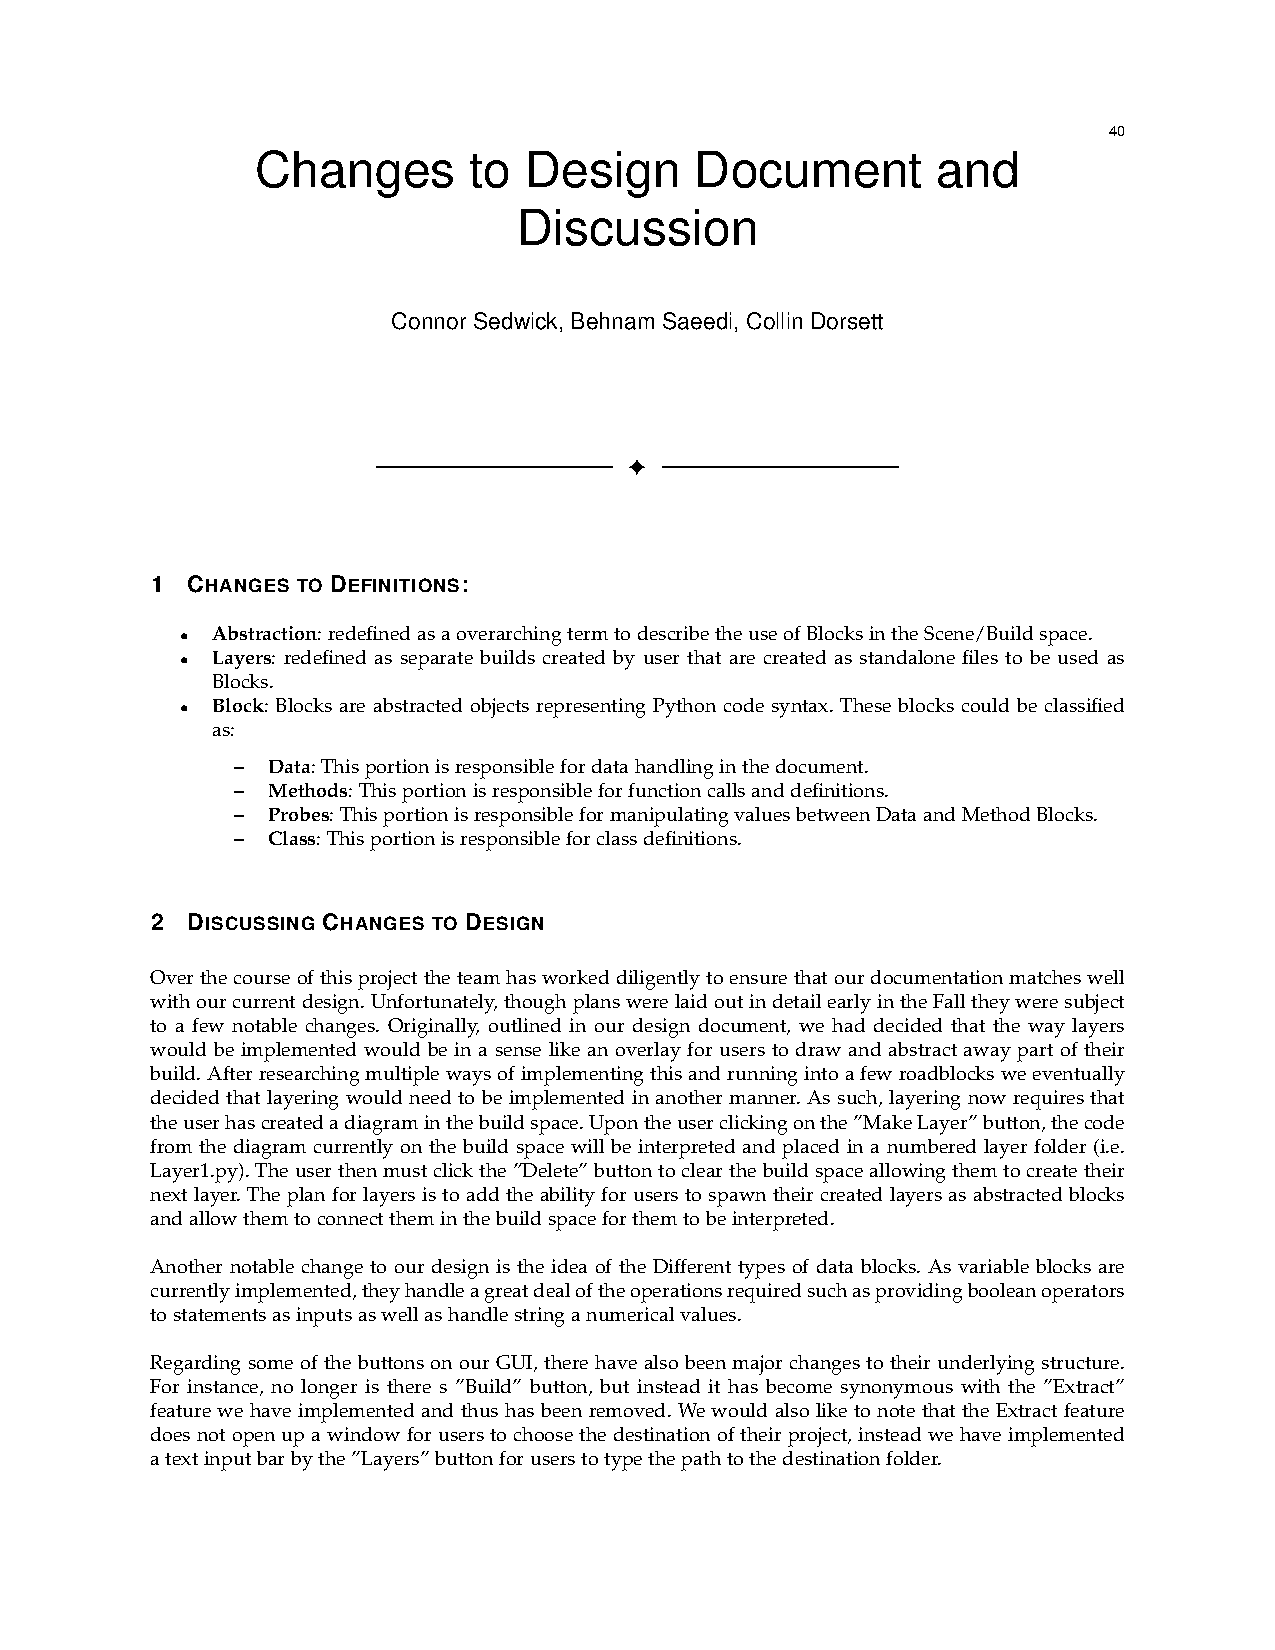
\includepdf[pages=1-, addtotoc={1,subsection,2,Design Document Discussion,Design Document Discussion}]{design-document-discussion}

\includepdf[pages=1-, addtotoc={1,section,1,Tech Review,Tech Review}]{visualflow-tech-review}
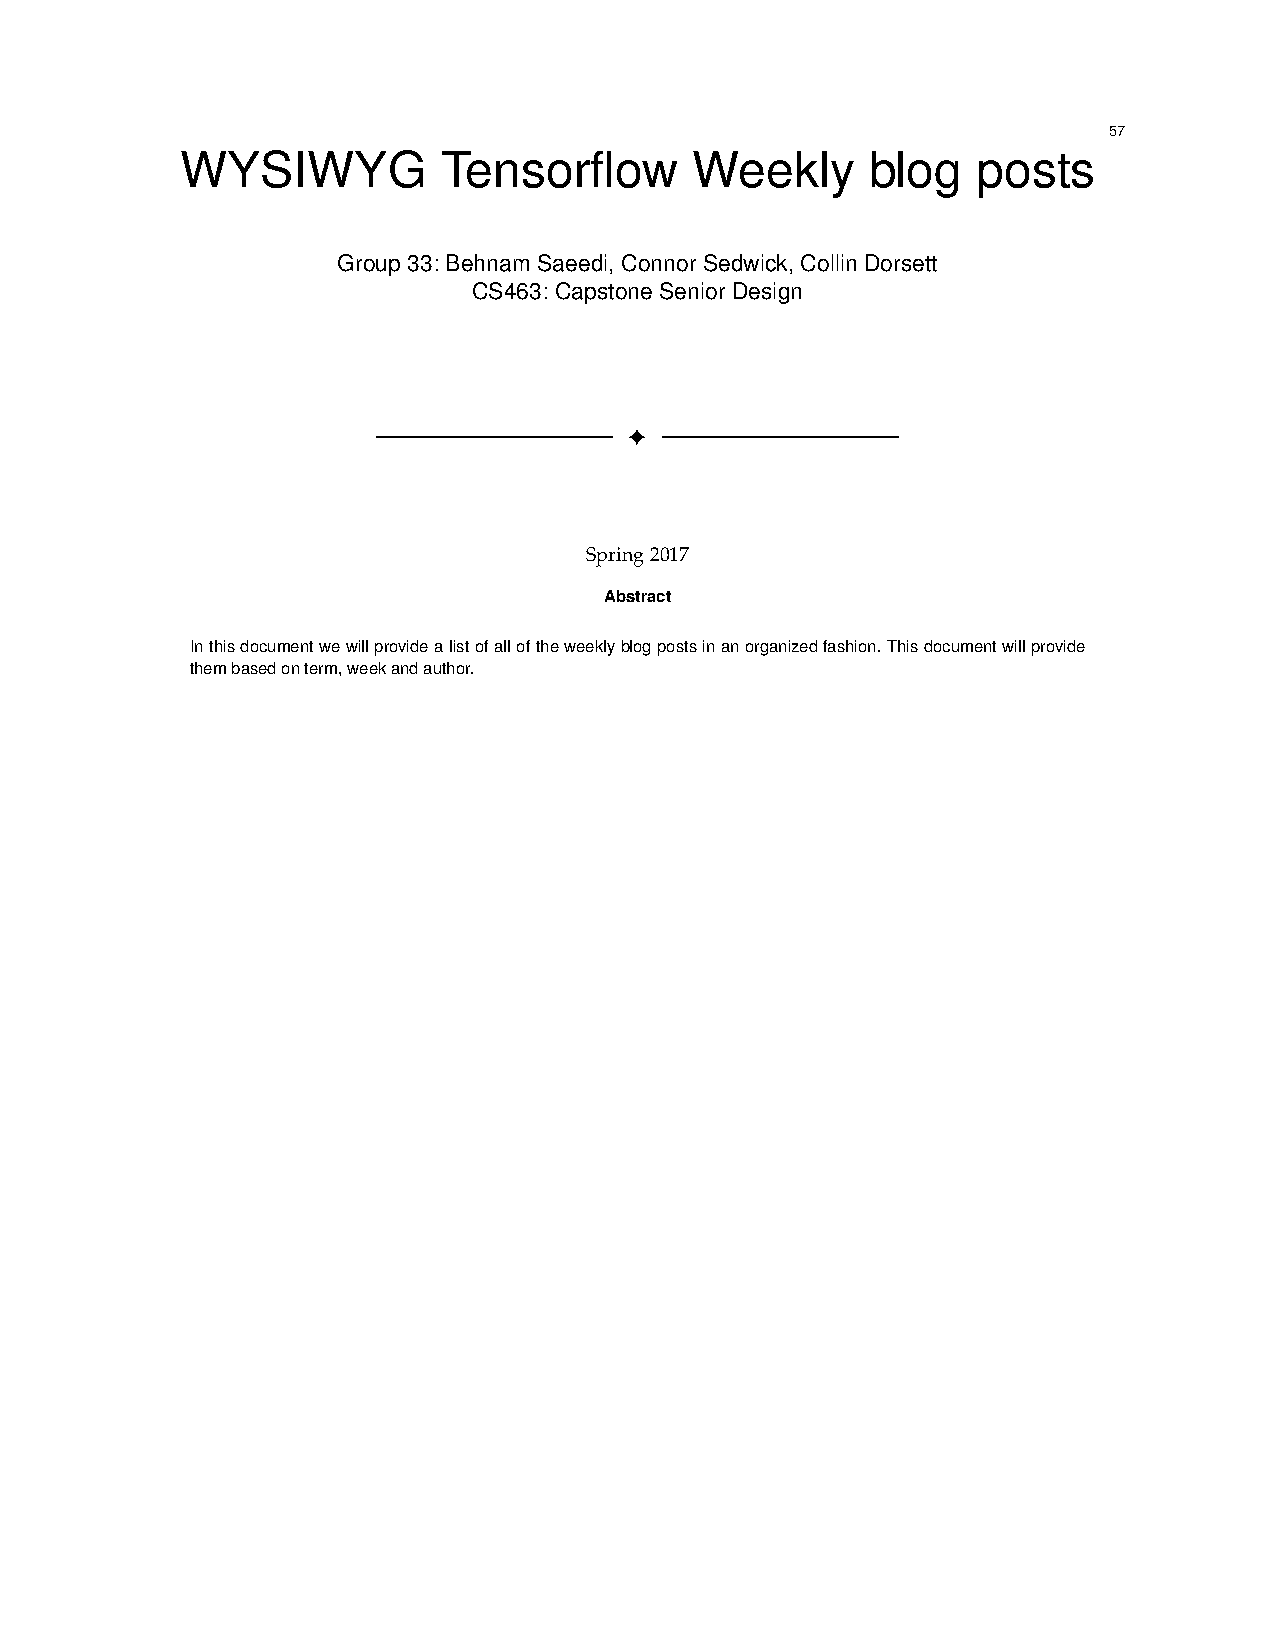
\includepdf[pages=1-, addtotoc={1,section,1,Blog Postings,Blog Postings}]{wysiwyg-tensorflow-weekly}

\includepdf[pages=1-, addtotoc={1,section,1,Manual,Manual}]{manual}
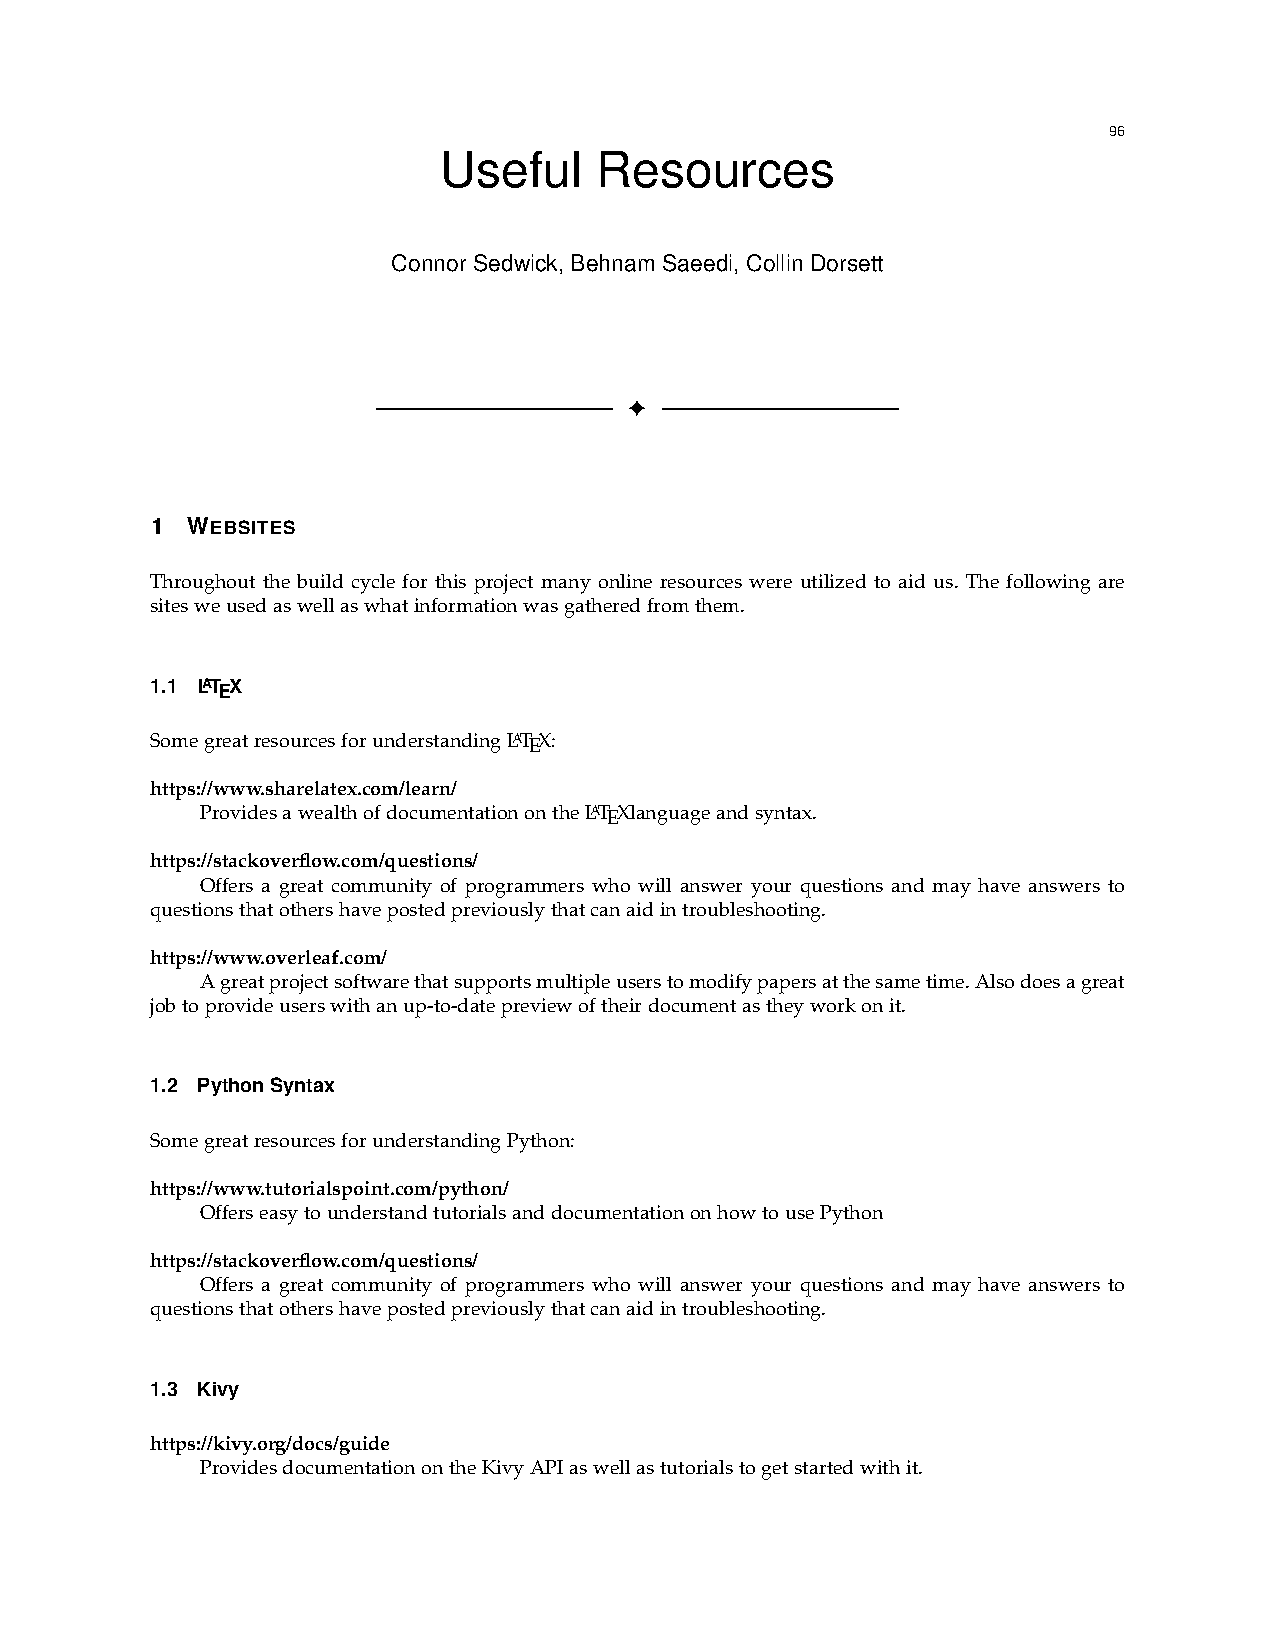
\includepdf[pages=1-, addtotoc={1,section,1,Resources,Resources}]{resources}
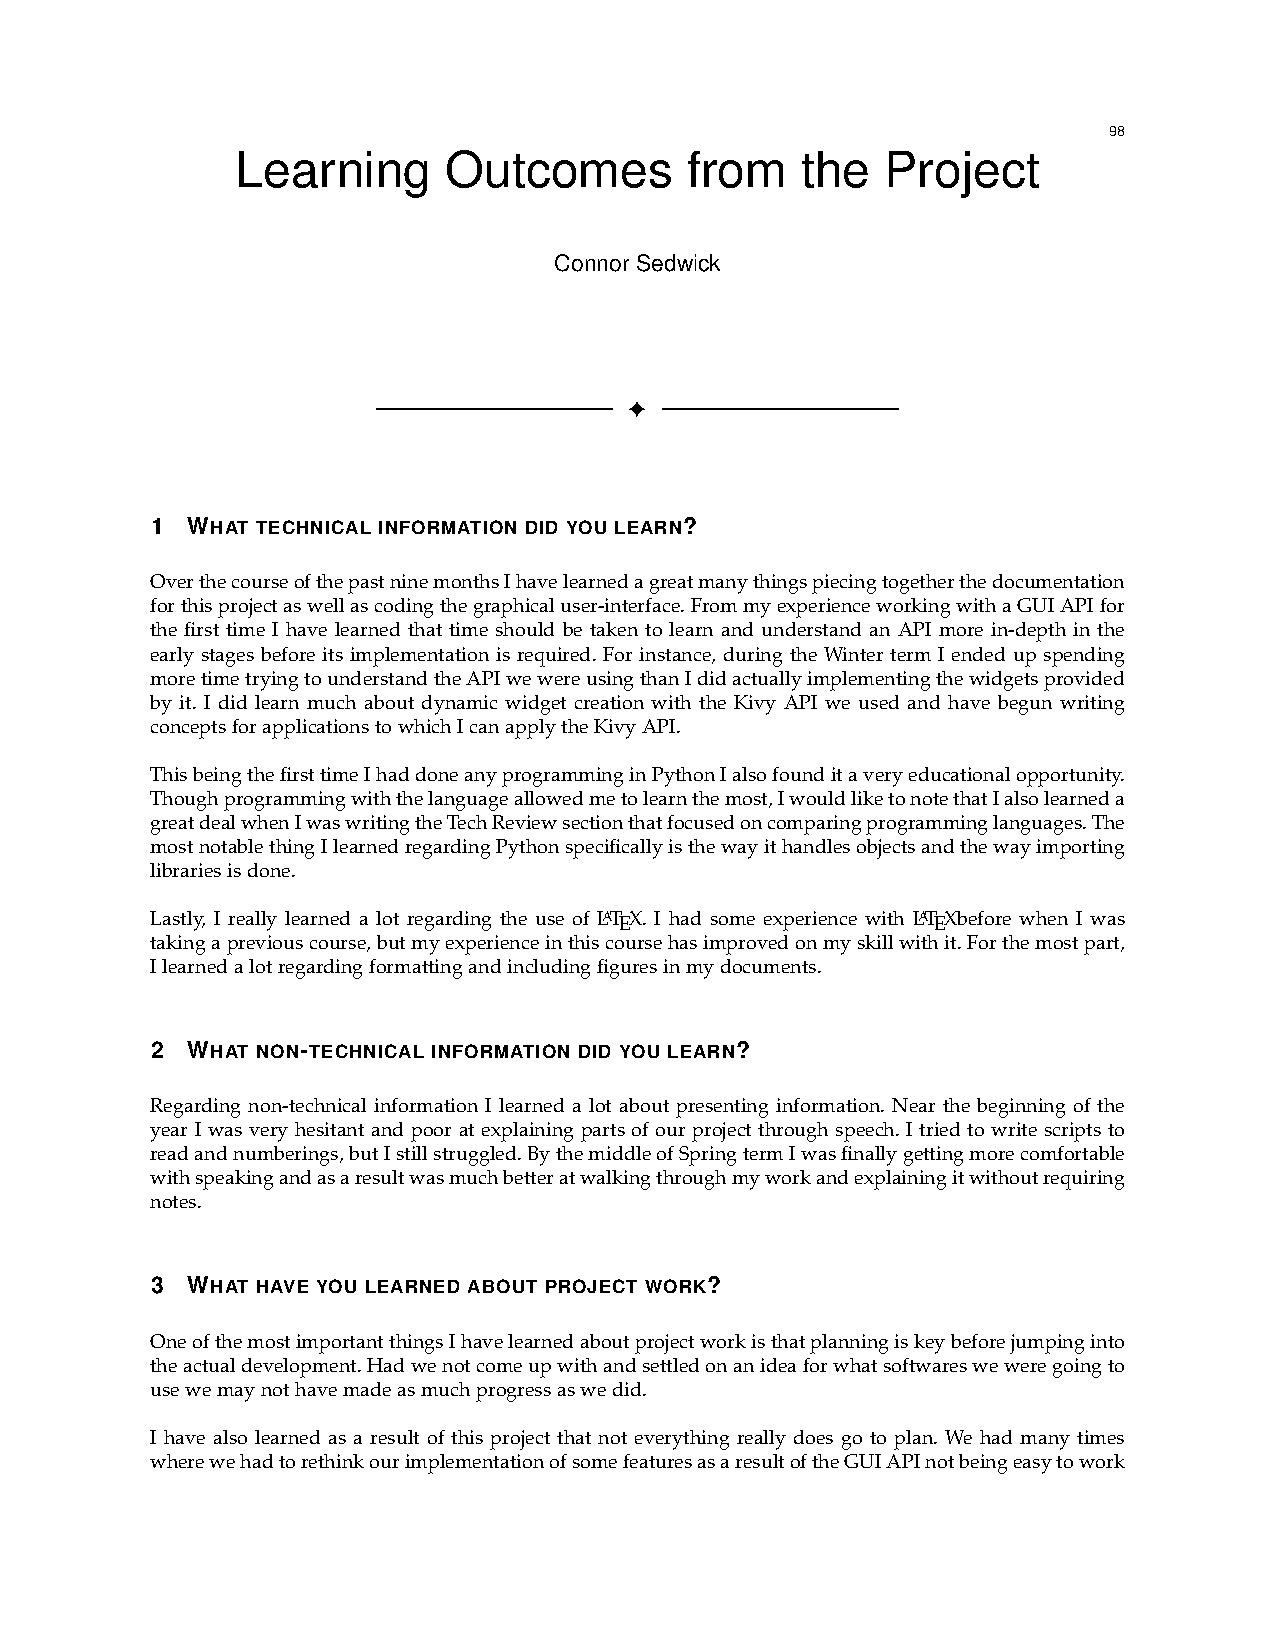
\includepdf[pages=1-, addtotoc={1,section,1,Connor's Learning Outcomes,Connor's Learning Outcomes}]{learning-outcomes-project_connor}
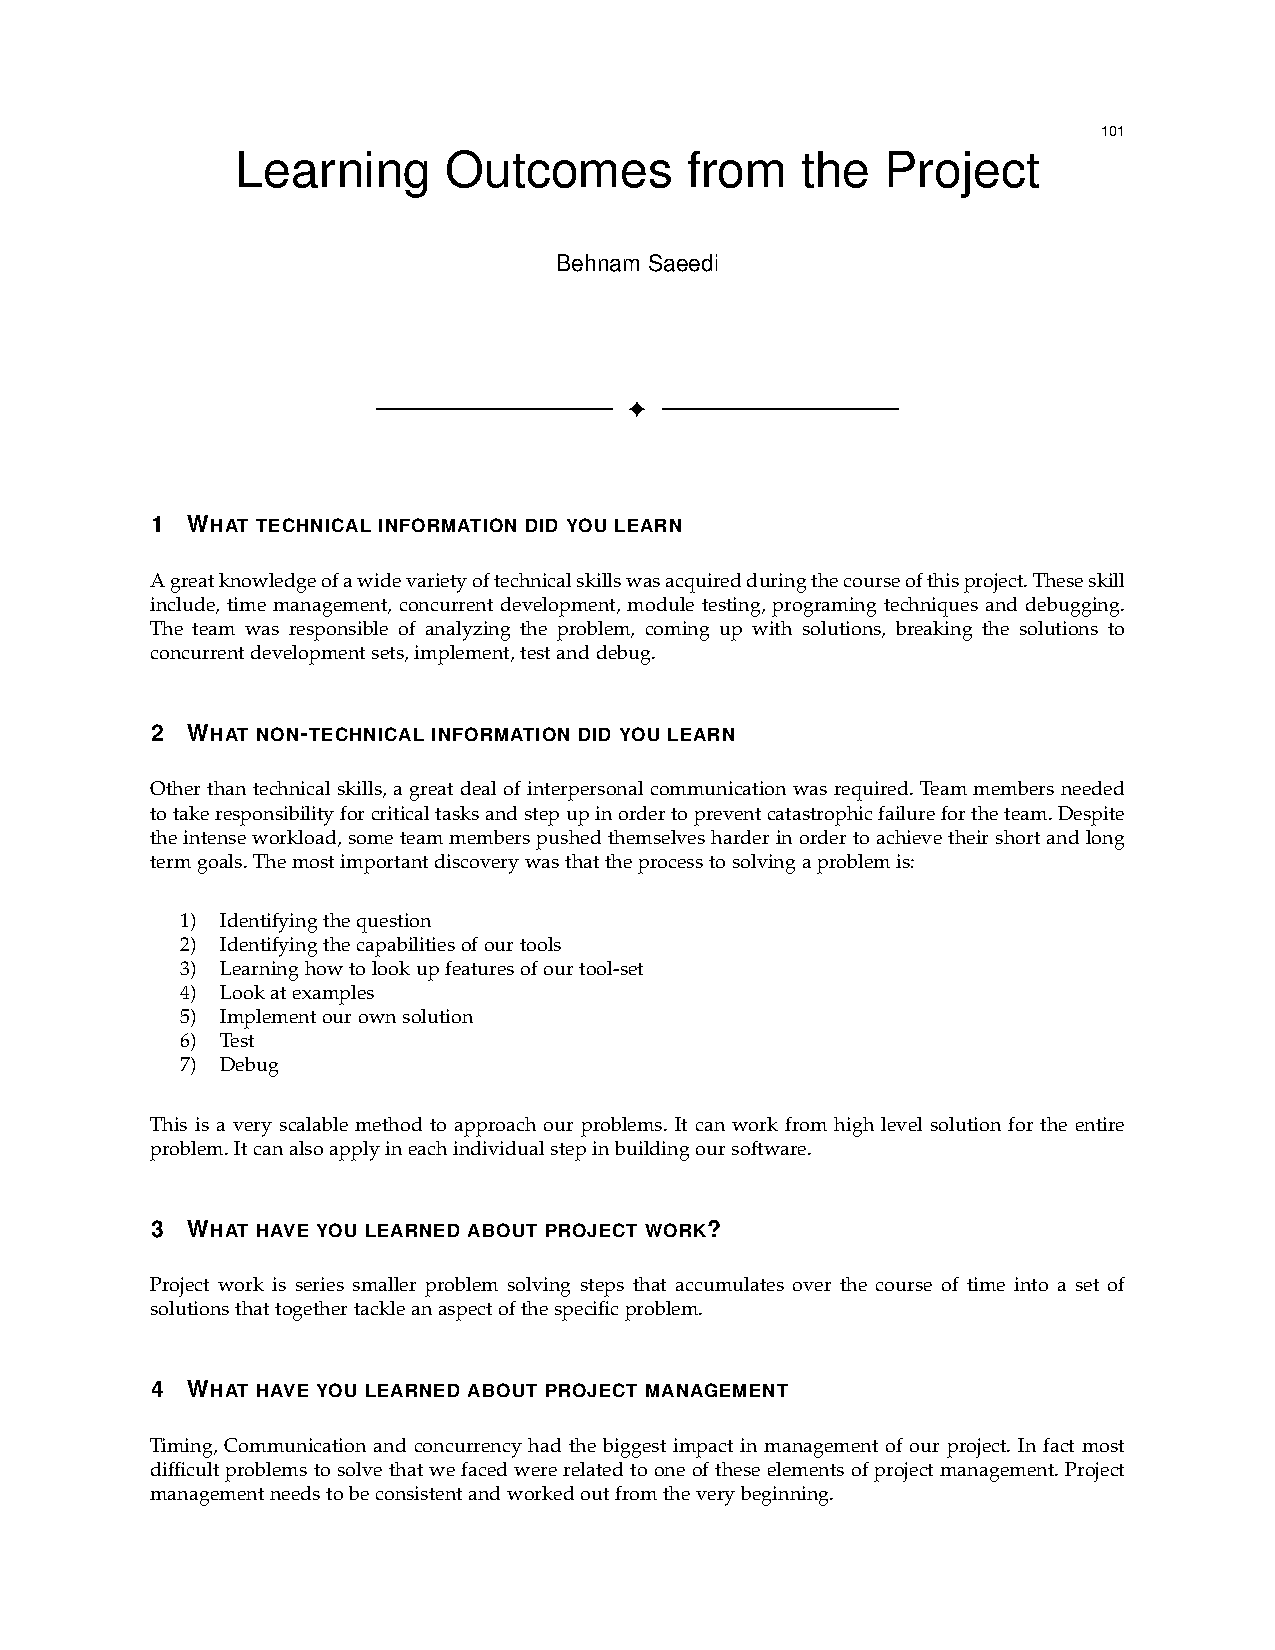
\includepdf[pages=1-, addtotoc={1,section,1,Behnam's Learning Outcomes,Behnam's Learning Outcomes}]{learning-outcomes-project-behnam}
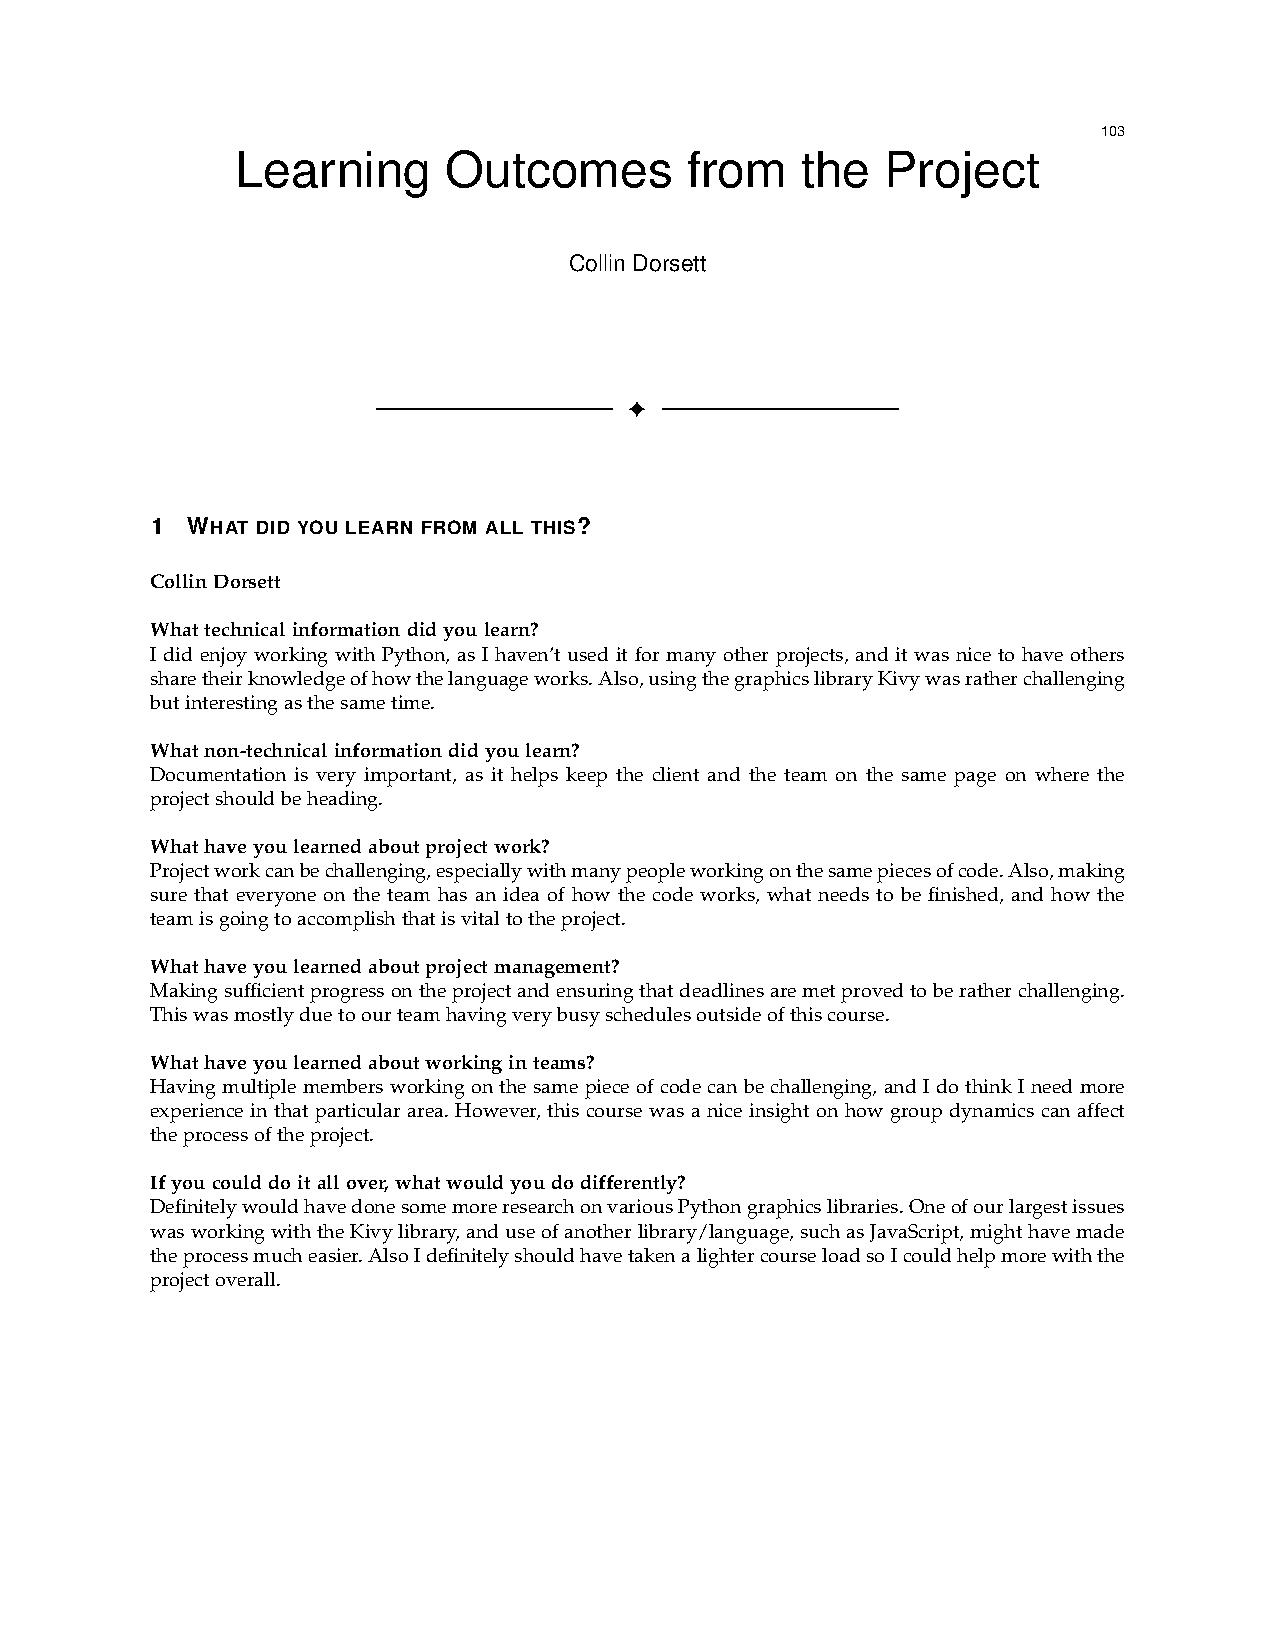
\includepdf[pages=1-, addtotoc={1,section,1,Collin's Learning Outcomes,Collin's Learning Outcomes}]{learning-outcomes-project-collin}

\includepdf[pages=1-, addtotoc={1,section,1,Appendix 1,Appendix 1}]{appendix-1}

\includepdf[pages=1-, addtotoc={1,section,1,Appendix 2,Appendix 2}]{appendix-2}
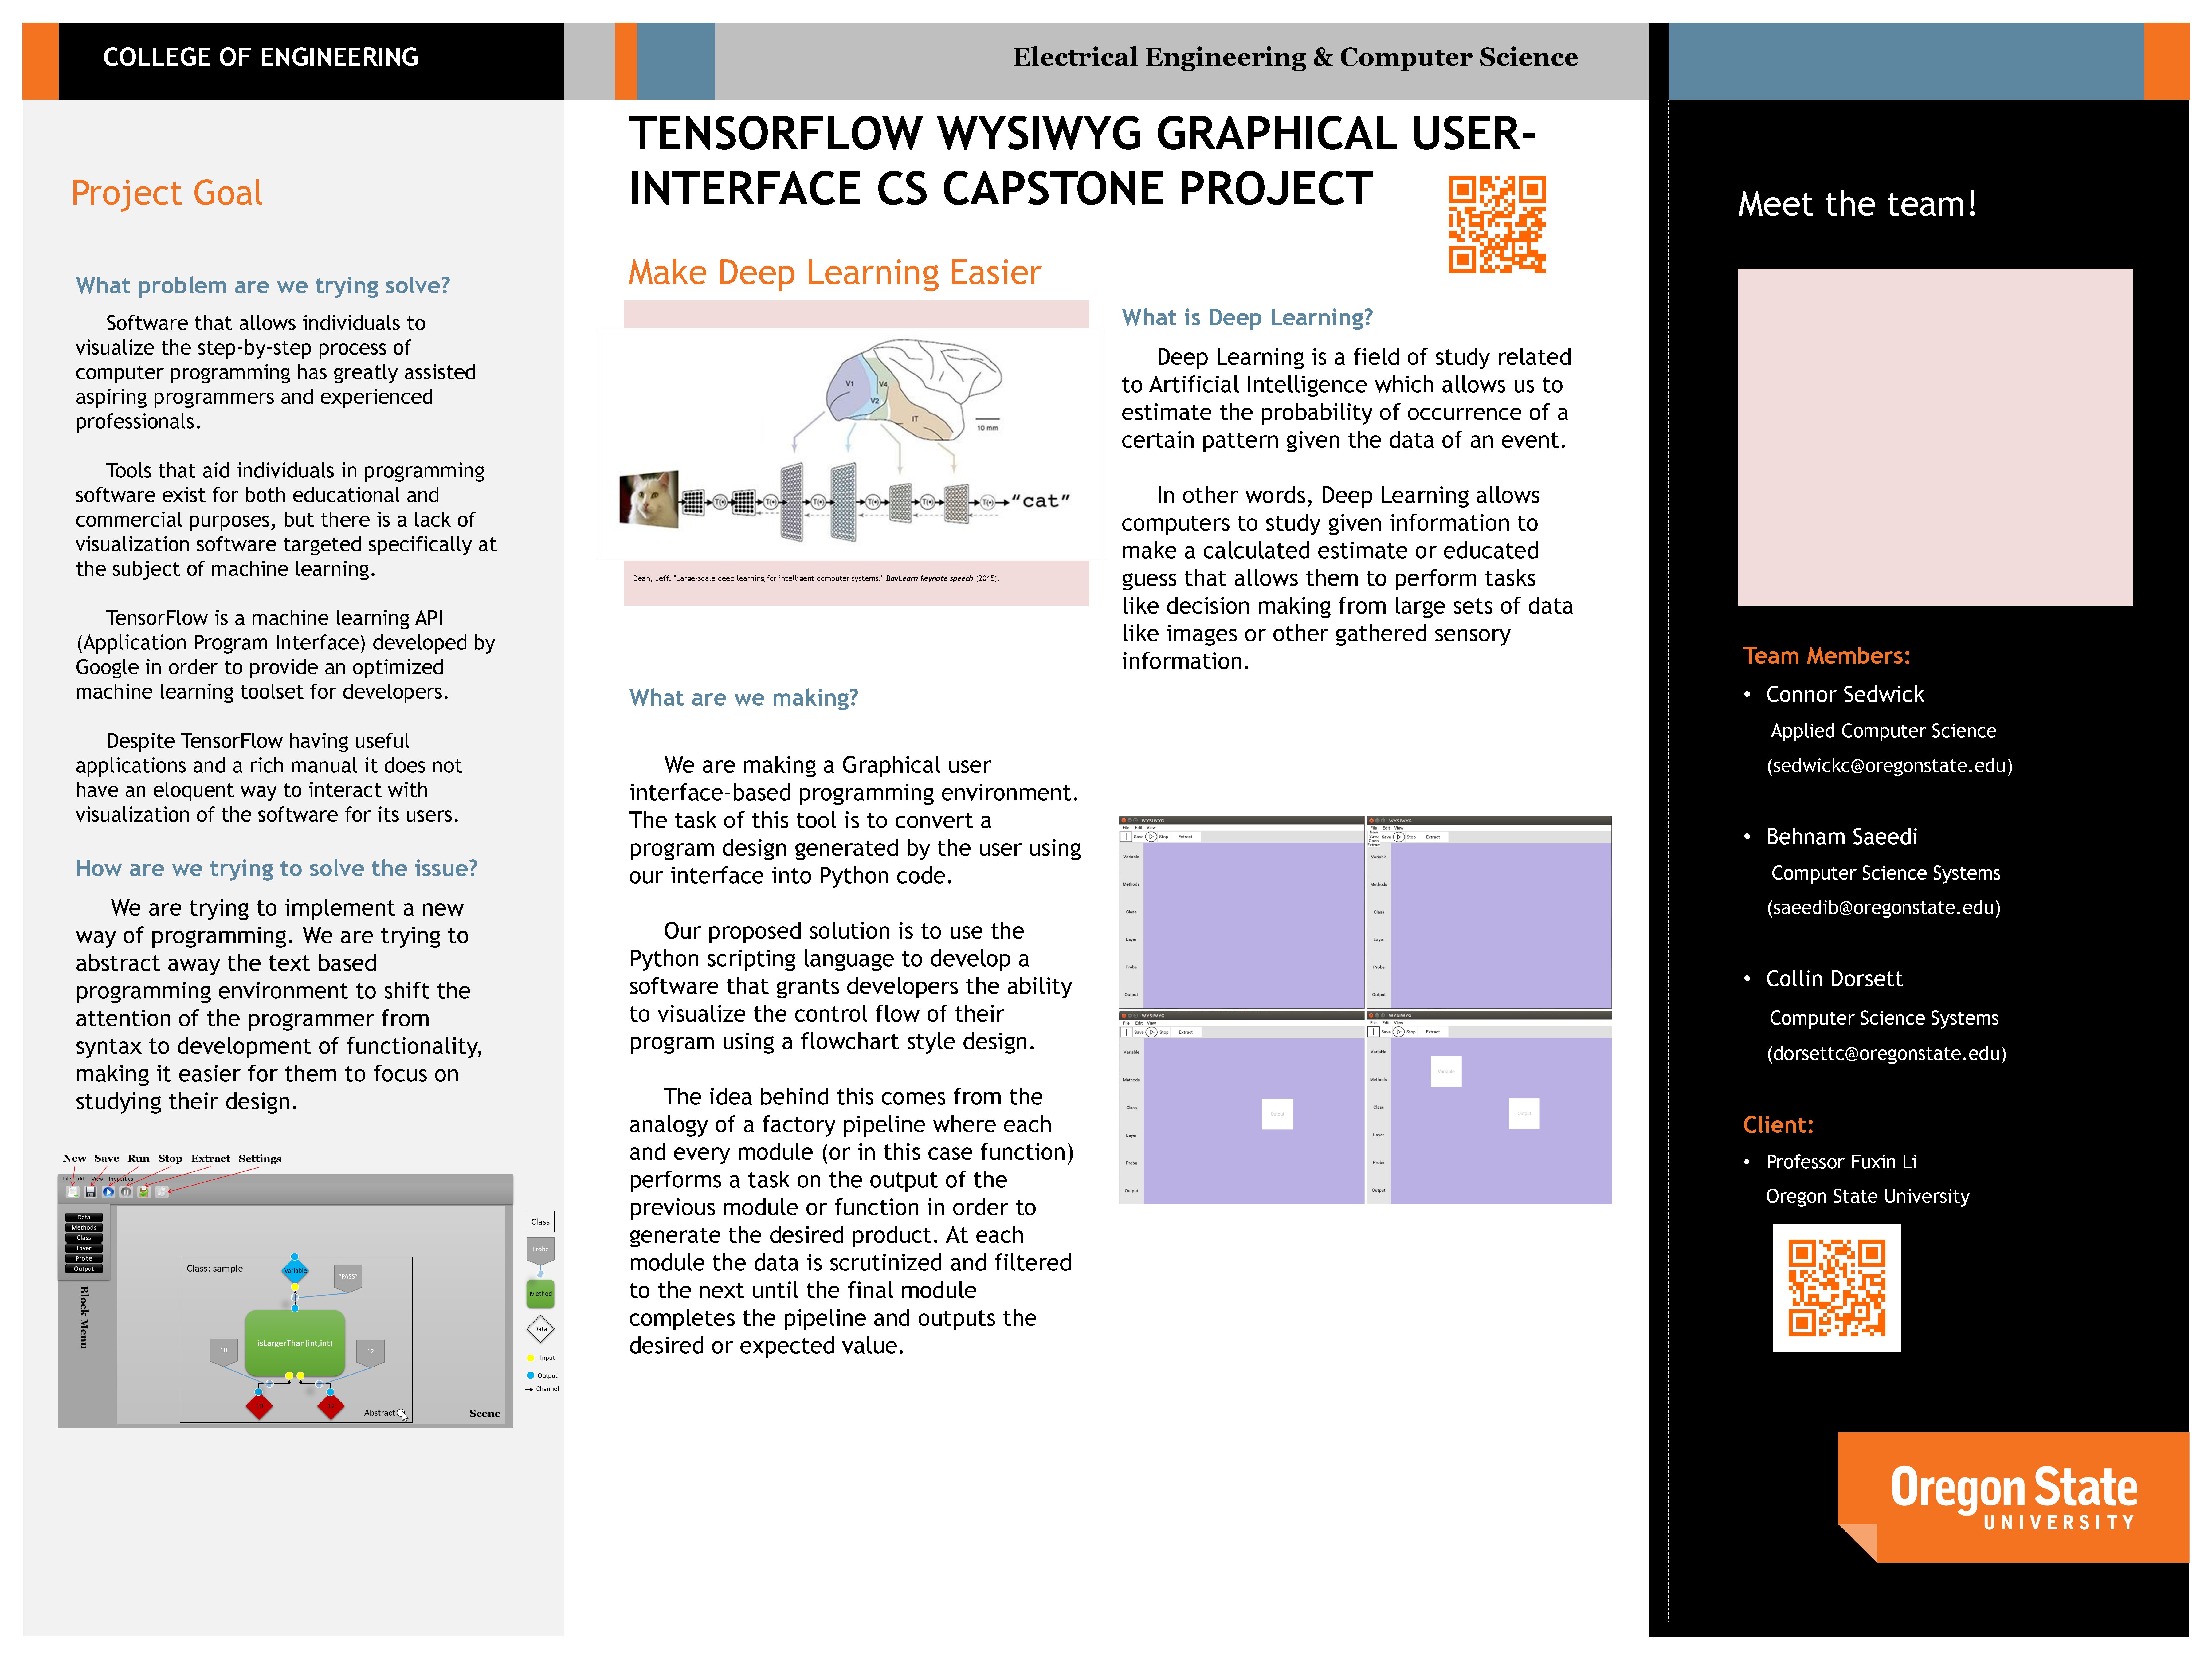
\includepdf[pages=1-, addtotoc={1,section,1,Team Poster, Team Poster}, angle=90]{team33}
\end{document}
